
\chapter{Interactive Paraphrasing}

Earlier we highlighted that during current project we considered paraphrasing as an interactive process. We considered interests of the end user by ensuring a real-time performance as well as by focusing on ranking for top paraphrasing candidates. In this chapter we introduce further work in this direction carried out by us during the project. We tweaked our interactive evaluation tool by adding UI elements that could be used to provide quick feedback on results. This feedback is instantly handled by our system in order to produce improved results. We also modified our automatic evaluation system in order to assess usability of this new feature.

\section{Handling user feedback}

Describing paraphrasing process, we introduced a method that uses a finite state machine to output a large number of paraphrasing suggestions. However, on the next steps this list is being filtered, sorted and only top 5 results are displayed to the user. All other paraphrasing options are wasted. Considering an interactive environment, we decided to introduce a UI feature that would let user to redefine his original query in light of the results he receives from the system. Receiving this feedback we go back to the output list and reorder it considering the feedback 

Inspired by relevance feedback concept from Information Retrieval field, we added buttons labeled ``Show More Like This'' near each paraphrase option in output screen. Clicking one of these buttons initiates a server request asking to update results by biasing them towards the corresponding paraphrase candidate. Figure 5.1 illustrates the updated UI. 

\begin{figure}
 \centering 
 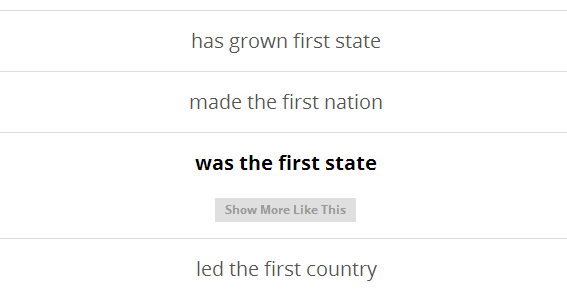
\includegraphics[scale=0.8]{g/show-more-like-this.png}
 \caption{``Show More Like This'' button}
\end{figure}

To implement this feature on the server-side, we simply developed a new sorter function, named \textbf{User Feedback Based Sorter} (\texttt{\textbf{UFBS}}). This sorter reorders final paraphrasing options list using string distance and word distance features as the primary and secondary weight functions. As a result, top items of the final are the most similar ones to the phrase specified in user feedback. 

In current implementation we re-run original query to retrieve the paraphrases list for feedback based sorting. However it's possible to implement this functionality in a more efficient way by saving results in cache, reusing them when user provides feedback. 

\section{Evaluation}

We modified our automatic evaluation process, by considering not only the original top results, but also results retrieved by providing each of the original paraphrasing option as user feedback. This way number of potential paraphrasing candidates dramatically increased. For our baseline approach we got \textbf{501} out of 2139 matches with desired paraphrase. Our best performing approach scored \textbf{847} out of 2139 test cases. 

However, the automatic evaluation considers that user will always provide useful feedback, which is not a realistic assumption. To test feasibility of the new feature, we carried out another small user study. Two participants were marking 30 same test cases using an updated version of our interactive evaluation tool. For baseline approach we got \textbf{11} cases in which at least one user found the desired paraphrase and \textbf{6} cases where both users found a suitable option. For the best approach these numbers are correspondingly \textbf{23} and \textbf{18}. Sign test confirmed significance of these results. Considering this outcome and comments from users, we conclude that the user feedback feature is really helpful in context of paraphrasing task.

\section{Specified paraphrasing requests}

Analysing the situations in which translator may want to use our paraphrasing tool, we found three core use cases:

\begin{itemize}
    \item User tries to find better wording for translation and wants to explore all options that express same meaning
    \item User expects to get a fixed version of an erroneous part in the translation
    \item User is not familiar with source language and machine translation does not seem to be good. Paraphrasing is used to understand what the selected part of translation means  
\end{itemize}

Furthermore, investigating each case in detail, we noticed that there are some other special cases when paraphrasing could be useful including:

\begin{itemize}
    \item Paraphrasing could be used to expand or collapse abbreviations. As we consider context of translation during paraphrasing this might be useful to find out correct meaning of a given abbreviation.

    \item Paraphrasing could be used to find out synonyms to a selected words in the translation. This is the main reason behind single word selection requests

    \item User might want to express same idea in a shorter or longer way, using more or less generic words. 
\end{itemize}

Considering all these situations, we designed another way of adding interactivity to our paraphrasing tool. This is done by introducing a smart ``Paraphrase'' button, which allows users to specify the main motivation behind their paraphrasing request. The button is implemented using a GUI component known as \emph{split button}, which represents a button with an arrow on the right side. Clicking the button will request default paraphrasing lookup. While clicking the arrow, will suggest more specific options based on the selection. Some use cases of the button are illustrated in Figure 5.2.   

\begin{figure}
 \centering 
 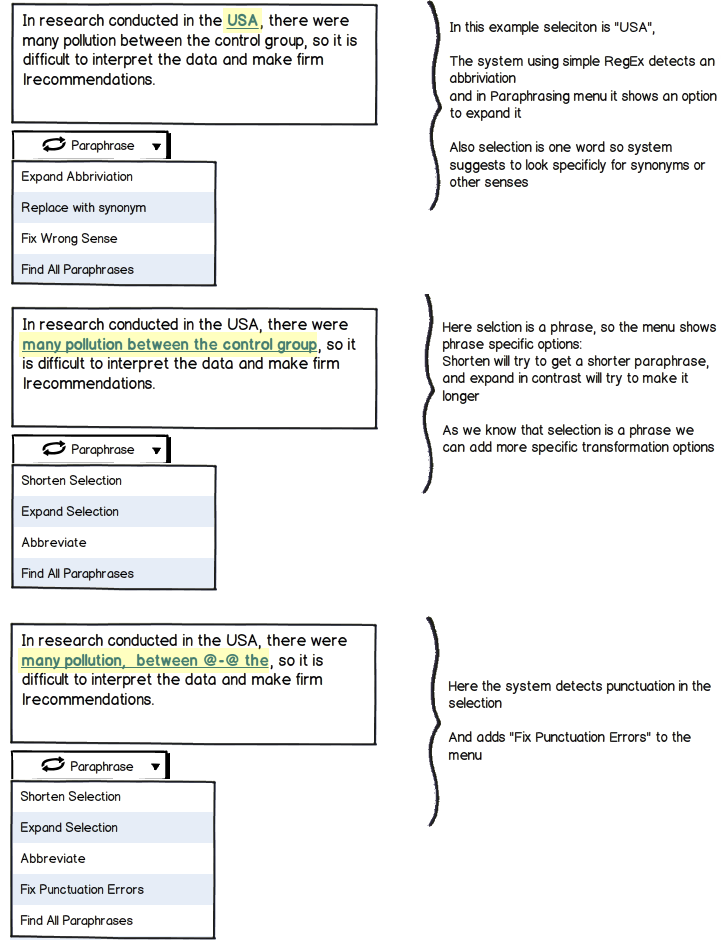
\includegraphics[scale=0.8]{g/button.png}
 \caption{``Paraphrase'' button}
\end{figure}

Similarly to user feedback functionality, these kind of specified queries are handled by introducing additional filters and sorters. In scope of this project we implemented only the ``expand abbreviation'' functionality as proof of the concept. The feature is supported by a filter that removes items where the first letters of each word doesn't follow the letters in original selection.
